\PassOptionsToPackage{table}{xcolor}
\documentclass{beamer}

\usepackage[utf8]{inputenc}
\usepackage{hyperref}
\usepackage{pgfpages}
\usepackage{dirtree}
\usepackage{tikz}
\usepackage{graphicx}
\usepackage{array}
\usepackage{tcolorbox}

\tcbset{%
	basic/.style={colframe=black,
		      colback=white,
		      top= 0mm,
		      bottom = 2mm,
		      boxsep=0mm
		      }
}

\usetikzlibrary{mindmap,calendar,backgrounds}
%\setbeameroption{hide notes}
\setbeamertemplate{note page}[plain]
\setbeameroption{show notes on second screen =left}
\AtEndNote{\vfill \begin{center} mm:hh \end{center}}
\newcommand{\notedir}[1] {
  \note{\dirtree{#1}}}
   
\makeatletter
\g@addto@macro{\endtabular}{\rowfont{}}% Clear row font
\makeatother
\newcommand{\rowfonttype}{}% Current row font
\newcommand{\rowfont}[1]{% Set current row font
   \gdef\rowfonttype{#1}#1%
}
\newcolumntype{L}{>{\rowfonttype}l}   
  
\definecolor{links}{HTML}{0000EE}
\hypersetup{colorlinks,linkcolor=,urlcolor=links}

\def \nom {Benjamin De Bruyne} %nom de l'étudiant-moniteur
\def \email {benjamin.debruyne@student.ulg.ac.be} %email de l'étudiant-moniteur

\title{Géométrie.}
    \author{\nom}
    \institute
    {
      Faculté des Sciences Appliquées.\\
      Université de Liège.
    }
    
    \date{Août 2017}
    
\begin{document}  
    \beamertemplatenavigationsymbolsempty
    
    \frame{\titlepage
	    \notedir{%
	      .1 Introduction.
	      .2 Mot d'accueil.
	      .2 Se présenter.
	      .3 Étudiant en ingénieur~civil..
	      .3 Réussi examen entrée..
	      .3 Viens pour donner trucs et astuces..      
	    }
	  }
    
    \frame{ \frametitle{Présentation du module.}
    
    \begin{figure}
     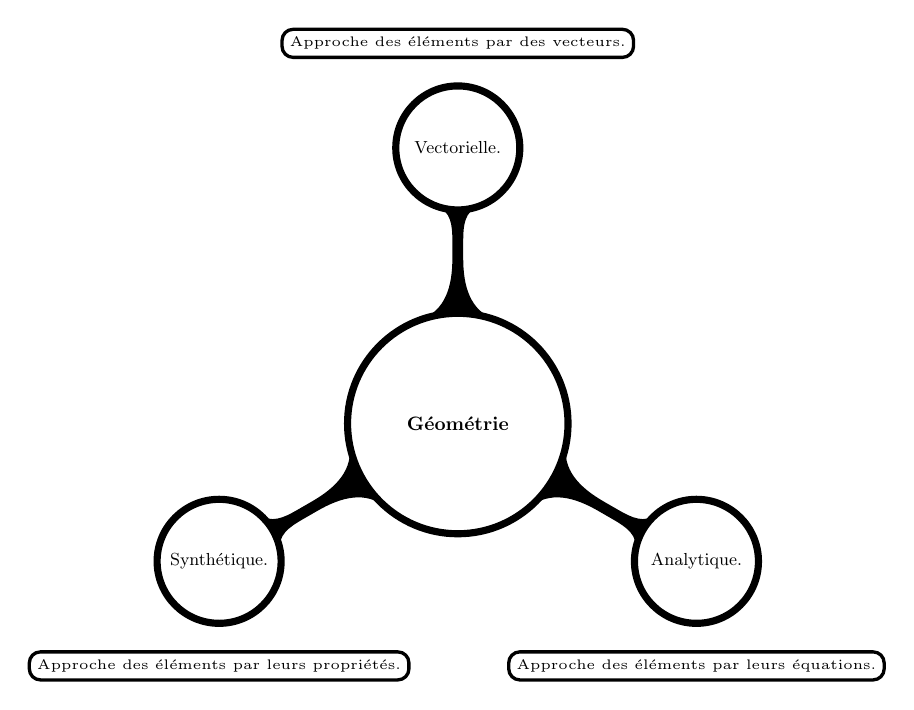
\begin{tikzpicture}[mindmap]
     
     \begin{scope}[
     every node/.style={concept,concept color=black, fill = white, line width = 0.6ex, text = black, execute at begin node=\hskip0pt,scale=0.7},
     %root concept/.append style={ concept color=black, fill = white, line width = 1ex, text = black},
     grow cyclic,
     level 1/.append style={level distance=3.5cm,sibling angle=120}]
   
    
     \node[font=\bfseries](Geometrie) {Géométrie} 
     [clockwise from=90]
     child { node (Vectorielle) {Vectorielle.}}
     child { node (Analytique) {Analytique.}}
     child { node (Synthetique) {Synthétique.}};
     \end{scope}
     \begin{scope}[every annotation/.style={concept, concept color=black,fill=white,text width={},align=center, rectangle}]
        \node[annotation,below,yshift=-10mm] at (Synthetique) {Approche des éléments par leurs propriétés.};
        \node[annotation,below,yshift=-10mm] at (Analytique) {Approche des éléments par leurs équations.};
        \node[annotation,above,yshift=10mm] at (Vectorielle) {Approche des éléments par des vecteurs.};
     \end{scope} 
     \end{tikzpicture}
    \end{figure}
   
    \notedir{%
    .1 Module de géométrie.
    .2 Vectorielle..
    .2 Synthétique..
    .2 Analytique.. 
    }
}
    \frame{\frametitle{Agenda.}
	  
	  \rowcolors{1}{white}{gray!10!}
	  \begin{tabular}{  L | L | L | L | L} 	 
	  \rowfont{\normalsize}%
	  \textmd{Jour} & \textmd{Horaire} & \textmd{Matière} & \textmd{Programme} & \textmd{Suggestion} \\ \hline
	  \rowfont{\scriptsize}%
	  \parbox[t]{1cm}{\textmd{Lundi}} & \textsl{8.45 - 12.15} & \parbox[t]{2.5cm}{Questions récentes;\\ Vectorielle.} & \parbox[t]{2.3cm}{\textit{15J1, 15J2, 16J1,
														 16J2; 01S3, 02S3,
														 03J3, 04J3, 04S3,
														 demo, bary, eule.}\\}
											     & \parbox[t]{2cm}{\textit{- ; 11J3, 13J3.}} \\  
	 \hline
	 \parbox[t]{1cm}{\textmd{Mercredi}} & \textsl{8.45 - 12.15} & \parbox[t]{2.5cm}{Synthétique plane;\\Synthétique espace.} & \parbox[t]{2.3cm}{\textit{01J1, 02J1, 03J1,
																			    03S1, supp; 01J4,
																			    01S4, 02S4, 11S5,
																			    12J5.} \\ 
														 }
											     & \parbox[t]{2cm}{\textit{13J1; 09S4.}} \\ 
											     \hline
	 \parbox[t]{1cm}{\textmd{Jeudi}} & \textsl{13.45 - 17.15} & \parbox[t]{2.5cm}{Analytique plan;\\ Analytique espace;\\ Questions récentes.} & \parbox[t]{2.3cm}{\textit{02J2, 02S2, 03J2,\\
													      03S2; 01J5, 01S5,
													      02J5, 03S5; 15S1, \\
													      15S2.\\
														 }}
											     & \parbox[t]{2cm}{\textit{11J2; 12J2; -.}} \\  
	 \parbox[t]{1cm}{\textmd{Vendredi}} & \textsl{15.30 - 17.15} & \parbox[t]{2.5cm}{Questions/Réponses.} & 
											     & 
	  \end{tabular}
	  \vfill \footnotesize
	  \rowcolors{1}{white}{white}
	  \begin{tabular}{l l l}
	   \textmd{Code exercice} :& xyMz &= 20xy \textmd{Mois Question z.} \\ \medskip
	   \textmd{Exemple} :& 15J1 &= 2015 \textmd{Juillet Question 1.}
	  \end{tabular}
	  \notedir{% 
	  .1 Agenda.
	  .2 Aujourd'hui.
	  .3 Questions des examens récents..
	  .3 Questions sur géométrie synthétique dans l'espace..
	  .2 Mercredi.
	  .3 Questions sur géométrie synthétique plane..
	  .3 Questions sur géométrie vectorielle..
	  .2 Jeudi.
	  .3 Questions sur géométrie analytique dans l'espace..
	  .3 Questions sur géométrie analytique plane..
	  .2 Vendredi.
	  .3 Séances de questions/réponses..
	  .4 Tous les encadrants des modules seront présents pour répondre de façon personnalisée à vos questions..
	  .2 Suggestion.
	  .3 Exercices à essayer à domicile après la séance..
	  } 
	  }
     \frame{ 
    \frametitle{Structures des résolutions.}
    \begin{columns}[t]
      \column{.5\textwidth}\centering
      \vspace{0pt}
      \begin{figure}
      \includegraphics[page=2,scale=0.35]{/home/bbruyne/Documents/Geometrie/PDF/sans_notes/Lecture_03/Recents/2015_Septembre_Q1.pdf} \\
      \includegraphics[page=3,scale=0.35]{/home/bbruyne/Documents/Geometrie/PDF/sans_notes/Lecture_03/Recents/2015_Septembre_Q1.pdf}
      \caption{\centering\scriptsize Géométrie synthétique et vectorielle.}
      \end{figure}
      
      \column{.5\textwidth}\centering
      \vspace{-1mm}
      \begin{figure}
      \includegraphics[page=2,scale=0.35]{/home/bbruyne/Documents/Geometrie/PDF/sans_notes/Lecture_03/Analytique_plan/2002_Juillet_Q2.pdf} \\
      \includegraphics[page=4,scale=0.35]{/home/bbruyne/Documents/Geometrie/PDF/sans_notes/Lecture_03/Analytique_plan/2002_Juillet_Q2.pdf}
      \caption{\centering\scriptsize Géométrie analytique.}
      \end{figure}
      
    \end{columns}
    \notedir{%
    .1 Structures.
    .2 Lecture énoncé.
    .3 Géométrie synthétique et vectorielle.
    .4 Accent sur hypothèses, thèse, dessin..
    .5 Favorise intuition..
    .3 Géométrie analytique.
    .4 Accent sur la découpe en sous-problèmes..
    .5 Permet de garder les idées claires..
    .2 Résolution.
    .3 Les 1,2,...~font références aux hypothèses numérotées..
    .3 Les théorèmes précédés d'un coeur sont à connaître..
    .3 Carré à la fin = cqfd..
    }
    }  
    \frame{
	   \frametitle{Liens utiles. (Cliquez sur le texte)}
	   \begin{enumerate}
	      \item{\href{http://www.facsa.ulg.ac.be/upload/docs/application/pdf/2012-07/geometrie_-_synthese.pdf}{Théorie}}, \\[0.8em]
	      \item{\href{http://www.montefiore.ulg.ac.be/~boigelot/cours/adm/}{Examens d'anciennes sessions}}, \\[0.8em]    
	      \item{Questions : \href{mailto:\email}{\email}}.
	   \end{enumerate} 	
	   \vfill \bigskip
	   Version 2017 des slides disponible sur : \\ \bigskip \centering 
	   \url{TODO}
	   \notedir{%
	   .1 Liens.
	   .2 Théorie.
	   .3 A consulter pour se rafraîchir l'esprit..
	   .3 Rappels théoriques seront faits..
	   .2 Anciens examens.
	   .3 Excellente préparation..
	   .4 Reprendre ses erreurs fréquentes sur feuille..
	   .2 Contact.
	   .3 Mieux comprendre notion théorique..
	   .3 Aide pour un exercice..
	   .3 Présent avant et après séances pour questions..
	   .2 Slides à disposition..
	   .3 Recopier url..
	   .3 Scanner QR code durant la pause..
	   }
	  }
	  
    
\end{document}

%%% Local Variables:
%%% mode: latex
%%% TeX-master: t
%%% End:
